\documentclass[]{project_report}
\usepackage{graphicx}
\usepackage[hidelinks ]{hyperref}
\usepackage{tikz}
\usepackage{doi}
\usepackage{hyperref}


%%%%%%%%%%%%%%%%%%%%%%
%%% Input project details
\def\studentname{Edward Instance}
\def\reportyear{2024}
\def\projecttitle{Advanced Web Development}
\def\supervisorname{Christos Dexiades}
\def\degree{BSc in Computer Science}
\def\fullOrHalfUnit{Full Unit} % indicate if you are doing the project as a Full Unit or Half Unit
\def\finalOrInterim{Project Plan} % indicate if this document is your Final Report or Interim Report

\begin{document}

\maketitle

%%%%%%%%%%%%%%%%%%%%%%
%%% Declaration

\chapter*{Declaration}

This report has been prepared on the basis of my own work. Where other published and unpublished source materials have been used, these have been acknowledged.

\vskip3em

Word Count: 2572 words

\vskip3em

Student Name: \studentname

\vskip3em

Date of Submission: 11/10/2024

\vskip3em

Signature: einstance

\newpage

%%%%%%%%%%%%%%%%%%%%%%
%%% Table of Contents
\tableofcontents\pdfbookmark[0]{Table of Contents}{toc}\newpage

%%%%%%%%%%%%%%%%%%%%%%
%%% Your Abstract here
\chapter*{Abstract}
\addcontentsline{toc}{chapter}{Abstract}

Online shopping has become an integral part of everyday life, with over 50 million users in the UK this year alone. This number is projected to rise by more than 10 million in the next five years \cite{statistica_2024}. Most online stores charge transaction fees for sales made on their platforms. For example, Amazon profits from transactions between third-party sellers and users \cite{zhu_2014}. While these fees are lucrative for the platform, they significantly reduce profit margins for sellers, particularly small-scale vendors with already tight margins, making it potentially detrimental. In addition to transaction fees, most payment gateways charge interchange, scheme, and processing fees. Usually, companies utilizing third-party payment systems incorporate the costs of these processing fees in the amounts charged for the subscriptions, and the end user hiring the services is the part covering all the costs, so companies can provide services while still profiting \cite{panov_2022}.

Instead of using these pricing models I am planning on using a subscription-based model, this would allow users to pay a monthly fee that would give them access to the application, but there are still some downfalls to this model. One of the key conditions for commercial success is the clearness and transparency of pricing \cite{laatikainen_2014} and there must be added value in subscription-based online services to make consumer feel that it is worth paying for \cite{wang_2024}. based on this I need to research other applications and be able to justify my pricing so that it is fair and competitive. I am planning on adding multiple levels to the model as solo users do not need the same amount of features as enterprise level users.

Some of the main functionality of the app includes, a user or group being able to sign-up to the application, then once they have paid for a subscription the user will be able to list items for sale and also post items. The user will be able to view their past payments, manage their account and more. There will also be admin pages both for managing user accounts but also for admins of the site to view data and analytics from the application. All of these features are essential to web applications, and there are more stretch goals that I am hoping to implement such as adding in a NoSQL database or a messaging system. All of these features will be considered and the ones that affect the user in the best way will be implemented.

The application will need to have a Role Based Access Control (RBAC) implemented to improve data security and to help manage users \cite{herzberg_2023} RBAC will be important to the project as it means that I will be able to grant users least privilege which means that a user or entity should only have access to the specific data, resources and applications needed to complete a required task \cite{palo_alto}. RBAC will also help me manage users as after assigning each user a role I can then easily change what they are allowed to see based on this role. 


I plan on researching a way to deploy this application either to a server or to a cloud provider, the main reason I am considering this is that because this is an online shop it will need to be deployed at some stage in the development so that users can access it. But I think it is important to think about this from the start so that the architecture can constantly evolve rather than leaving it late in the project and having to plan and provision it near the end of the project. The reason I am debating both types of deployments are that there are both advantages and disadvantages to either options. The main difference with the two is that you trade fixed expense for variable expense \cite{whitepaper_2024} when working with the cloud, as you don't have to pay the upfront cost for the servers.

I think this approach is important as it prioritises the users over making money, I think a user centered design and approach to creating this project will elevate it while also providing real world challenges that developers face. As well as that, the amount of features that a online store requires that I have mentioned will help me create a unique project where I can use both technologies I've learnt about but also new ones.

\newpage

%%%%%%%%%%%%%%%%%%%%%%
%%% Introduction
\chapter{Timeline}


I plan to spend the beginning of term one working on my project plan and deciding on the technologies and frameworks that I will be using. Then I will start building my application, I will be focusing on the Web and Application tier's as the data model will be defined based on them. I am hoping to have an Minimum viable product (MVP) by the end of week 8 so that I have time to test it and create my interim report by the end of week 10. After the report is submitted and I have completed the presentation I am planning to re-evaluate my plan for term 2, I am also planning to do a review in week 6 to ensure that I am on track and to help me prioritise work.

While there is an outline for a timeline for term 2 there is a high chance that this could change, and my plan to work around this is to consistently going back to the plan and timeline and reviewing where I am, what has changed and what I can approve so that even if I go off track I will be fine.


Across the two terms the main thing I want to focus on is splitting my focus between both the reports I need to create and the code as they both play important roles in the project.

\section{Term 1}


\begin{center}
    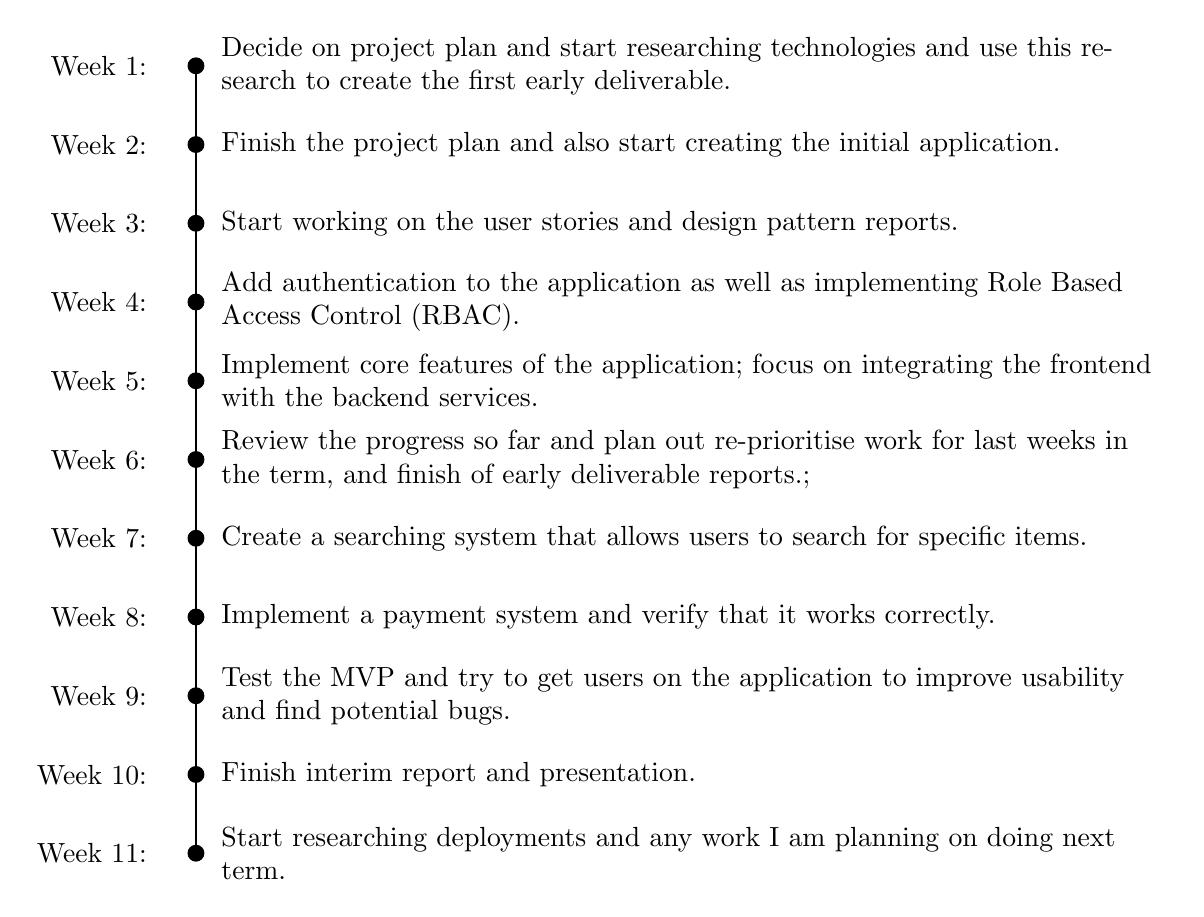
\begin{tikzpicture}[scale=1, every node/.style={scale=1}]

        \def\yshift{-1}  % Adjust the shift for better spacing
        % Draw the vertical timeline
        \draw[thick] (0,-1) -- (0,-11);  % Timeline from 0 to -10
        
        % Create the weeks and the dots for them
        \node[anchor=east] at (-0.5,\yshift) {Week 1:};
        \node[anchor=west, text width=12cm] at (0.2,\yshift) {Decide on project plan and start researching technologies and use this research to create the first early deliverable.};
        \draw[fill] (0,\yshift) circle (0.1);  

        \node[anchor=east] at (-0.5,2*\yshift) {Week 2:};
        \node[anchor=west, text width=12cm] at (0.2,2*\yshift) {Finish the project plan and also start creating the initial application.};
        \draw[fill] (0,2*\yshift) circle (0.1);  

        \node[anchor=east] at (-0.5,3*\yshift) {Week 3:};
        \node[anchor=west, text width=12cm] at (0.2,3*\yshift) {Start working on the user stories and design pattern reports.};
        \draw[fill] (0,3*\yshift) circle (0.1);  

        \node[anchor=east] at (-0.5,4*\yshift) {Week 4:};
        \node[anchor=west, text width=12cm] at (0.2,4*\yshift) {Add authentication to the application as well as implementing Role Based Access Control (RBAC).};
        \draw[fill] (0,4*\yshift) circle (0.1);  

        \node[anchor=east] at (-0.5,5*\yshift) {Week 5:};
        \node[anchor=west, text width=12cm] at (0.2,5*\yshift) {Implement core features of the application; focus on integrating the frontend with the backend services.};
        \draw[fill] (0,5*\yshift) circle (0.1);  

        \node[anchor=east] at (-0.5,6*\yshift) {Week 6:};
        \node[anchor=west, text width=12cm] at (0.2,6*\yshift) {Review the progress so far and plan out re-prioritise work for last weeks in the term, and finish of early deliverable reports.;};
        \draw[fill] (0,6*\yshift) circle (0.1);  

        \node[anchor=east] at (-0.5,7*\yshift) {Week 7:};
        \node[anchor=west, text width=12cm] at (0.2,7*\yshift) {Create a searching system that allows users to search for specific items.};
        \draw[fill] (0,7*\yshift) circle (0.1);  

        \node[anchor=east] at (-0.5,8*\yshift) {Week 8:};
        \node[anchor=west, text width=12cm] at (0.2,8*\yshift) {Implement a payment system and verify that it works correctly.};
        \draw[fill] (0,8*\yshift) circle (0.1);  

        \node[anchor=east] at (-0.5,9*\yshift) {Week 9:};
        \node[anchor=west, text width=12cm] at (0.2,9*\yshift) {Test the MVP and try to get users on the application to improve usability and find potential bugs.};
        \draw[fill] (0,9*\yshift) circle (0.1);  

        \node[anchor=east] at (-0.5,10*\yshift) {Week 10:};
        \node[anchor=west, text width=12cm] at (0.2,10*\yshift) {Finish interim report and presentation.};
        \draw[fill] (0,10*\yshift) circle (0.1);  
        
        \node[anchor=east] at (-0.5,11*\yshift) {Week 11:};
        \node[anchor=west, text width=12cm] at (0.2,11*\yshift) {Start researching deployments and any work I am planning on doing next term.};
        \draw[fill] (0,11*\yshift) circle (0.1);  

    \end{tikzpicture}
\end{center}




\section{Term 2}


\begin{center}
    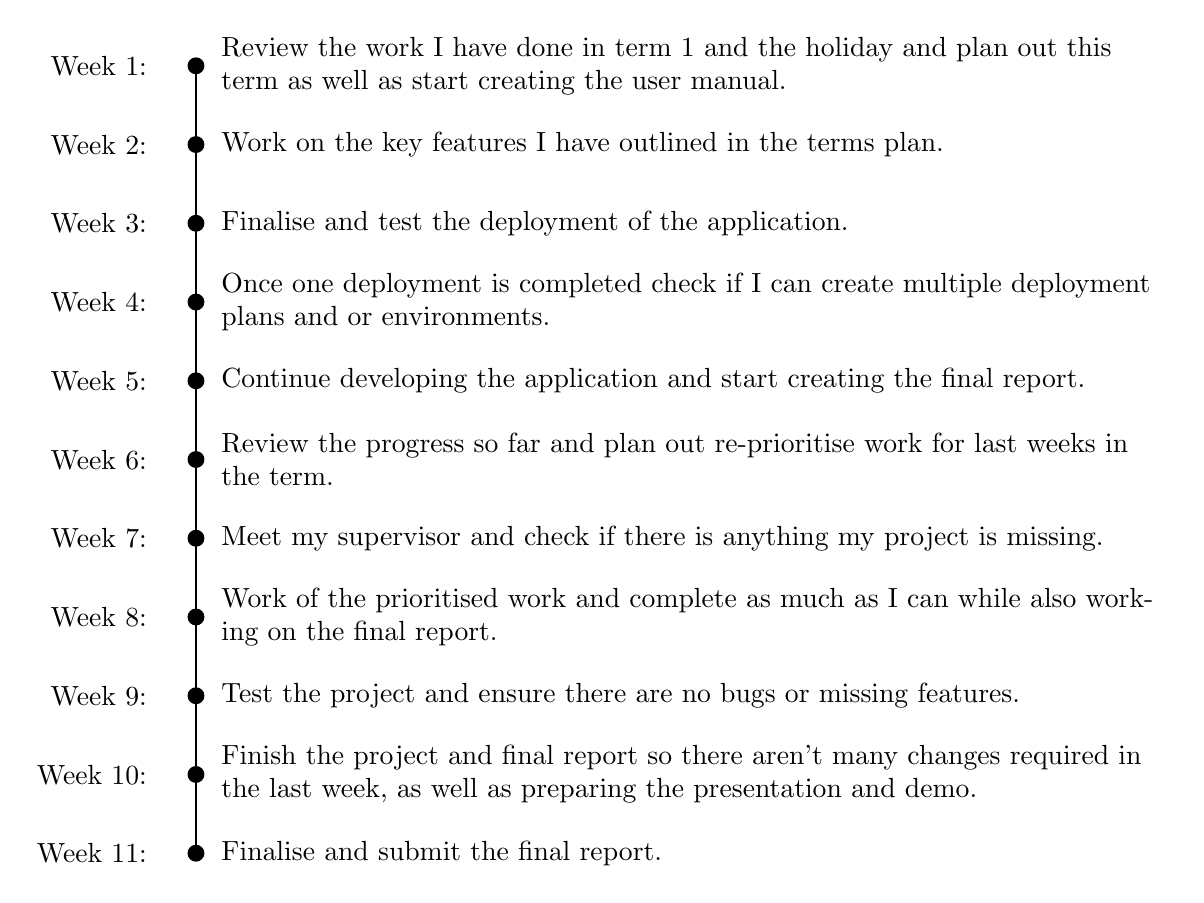
\begin{tikzpicture}[scale=1, every node/.style={scale=1}]

        \def\yshift{-1}  % Adjust the shift for better spacing
        % Draw the vertical timeline
        \draw[thick] (0,-1) -- (0,-11);  % Timeline from 0 to -10
        
        % Create the weeks and the dots for them
        \node[anchor=east] at (-0.5,\yshift) {Week 1:};
        \node[anchor=west, text width=12cm] at (0.2,\yshift) {Review the work I have done in term 1 and the holiday and plan out this term as well as start creating the user manual.};
        \draw[fill] (0,\yshift) circle (0.1);  

        \node[anchor=east] at (-0.5,2*\yshift) {Week 2:};
        \node[anchor=west, text width=12cm] at (0.2,2*\yshift) {Work on the key features I have outlined in the terms plan.};
        \draw[fill] (0,2*\yshift) circle (0.1);  

        \node[anchor=east] at (-0.5,3*\yshift) {Week 3:};
        \node[anchor=west, text width=12cm] at (0.2,3*\yshift) {Finalise and test the deployment of the application.};
        \draw[fill] (0,3*\yshift) circle (0.1);  

        \node[anchor=east] at (-0.5,4*\yshift) {Week 4:};
        \node[anchor=west, text width=12cm] at (0.2,4*\yshift) {Once one deployment is completed check if I can create multiple deployment plans and or environments.};
        \draw[fill] (0,4*\yshift) circle (0.1);  

        \node[anchor=east] at (-0.5,5*\yshift) {Week 5:};
        \node[anchor=west, text width=12cm] at (0.2,5*\yshift) {Continue developing the application and start creating the final report.};
        \draw[fill] (0,5*\yshift) circle (0.1);  

        \node[anchor=east] at (-0.5,6*\yshift) {Week 6:};
        \node[anchor=west, text width=12cm] at (0.2,6*\yshift) {Review the progress so far and plan out re-prioritise work for last weeks in the term.};
        \draw[fill] (0,6*\yshift) circle (0.1);  

        \node[anchor=east] at (-0.5,7*\yshift) {Week 7:};
        \node[anchor=west, text width=12cm] at (0.2,7*\yshift) {Meet my supervisor and check if there is anything my project is missing.};
        \draw[fill] (0,7*\yshift) circle (0.1);  

        \node[anchor=east] at (-0.5,8*\yshift) {Week 8:};
        \node[anchor=west, text width=12cm] at (0.2,8*\yshift) {Work of the prioritised work and complete as much as I can while also working on the final report.};
        \draw[fill] (0,8*\yshift) circle (0.1);  

        \node[anchor=east] at (-0.5,9*\yshift) {Week 9:};
        \node[anchor=west, text width=12cm] at (0.2,9*\yshift) {Test the project and ensure there are no bugs or missing features.};
        \draw[fill] (0,9*\yshift) circle (0.1);  

        \node[anchor=east] at (-0.5,10*\yshift) {Week 10:};
        \node[anchor=west, text width=12cm] at (0.2,10*\yshift) {Finish the project and final report so there aren't many changes required in the last week, as well as preparing the presentation and demo.};
        \draw[fill] (0,10*\yshift) circle (0.1);  
        
        \node[anchor=east] at (-0.5,11*\yshift) {Week 11:};
        \node[anchor=west, text width=12cm] at (0.2,11*\yshift) {Finalise and submit the final report.};
        \draw[fill] (0,11*\yshift) circle (0.1);  

    \end{tikzpicture}
\end{center}



\chapter{Risks and Mitigation's}

\section{GDPR (General Data Protection Regulation) Concerns}

The risk here is failing to meet standards set by GDPR, failing to meet these standards can occur warnings, fines up to £20 million or 4\% of the business’s total annual worldwide turnover and potential bans on processing \cite{europeancommission_2023}. I have researched some of the main policies that an online shop should meet and how I plan to mitigate the overall risk of not meeting standards.

\subsection{Data Collection and Consent}

GDPR requires not only that data is only collected after obtaining consent from the user, but also that data is collected and used only for specific purposes, and must be deleted when those purpose are no longer applicable \cite{basin_2018}. To ensure compliance, I will obtain explicit user consent before collecting personal data, based on the conditions for consent \cite{gdpr_2016}[Article 7 ].

\subsection{Data Minimisation}

“[Personal data shall be] adequate, relevant and limited to what is necessary in relation to the purposes for which they are processed [...]” \cite{gdpr_2016} [Article 5, Sect. 1(c)]. Therefore only the necessary data for the service will be collected, in order to comply with the principle of data minimisation. I will also occasionally review what data I am collecting and if it is required.

\subsection{Data Security}

The controller and the processor shall implement appropriate technical and organisational measures to ensure a level of security appropriate to the risk \cite{gdpr_2016} [Article 32, Sect. 1]. To ensure a good level of data security throughout the project I will research and implement best practices.

\subsection{Data Retention}

Data should not be stored no longer than is necessary for the purposes for which the personal data are processed \cite{gdpr_2016} [Article 5, Sect. 1(e)]. To mitigate this risk a clear data retention policy will be enforced, ensuring that personal data is not stored longer than necessary and data that is no longer needed will be securely deleted.

\subsection{User Rights}

Mechanisms will be in place to allow users to exercise their rights under GDPR which are listed here \cite{gdpr_2016} [Chapter 3], including access to their data, the right to rectification, and the right to be forgotten.

\subsection{Third Parties}

Any third-party services used, such as payment gateways, authentication providers and more will be GDPR compliant. To ensure this I will look into documentation and check their policies. \newline

All of these GDPR policies affect the web application I will be building and the mitigation to them is to ensure that when any user data is being used or requested to make sure that it is for a reason, and to also have a plan on how to deal with data security and knowing what I might need to implement into the project as I have identified this risk. This risk has a low likelihood and a high severity as these data risks are very important and could cause lot of issues, it is easy to mitigate them by planning and preparing.


\section{Security Risks}

There are many security risks when it comes to web applications and each of these require different solutions. My plan is to mitigate these vulnerabilities by focusing on the Open Worldwide Application Security Project (OWASP) Top Ten Web Application Security Risks \cite{owasp_2021}. This list highlights the most common and severe risks, which are frequently exploited by attackers, and thus have a high likelihood of being targeted. In addition to addressing these known vulnerabilities, I will continue to check for new risks as I progress. This risk is both a high likelihood and severity risk as any security risks can be detrimental to the application and they are very likely as 50\% of UK businesses experienced some form of cyber attack in 2023 \cite{griffiths_2023}.


\section{Scalability Issues}

As the application grows and creates a large user base there are issues related to scaling, if there are too many users for the application it could create unknown errors and potentially deny users access to the application. To mitigate this I plan to add load balancing and auto-scaling to the deployment steps, this should insure that the application will be able to handle increased and spiked traffic. This risk would be a high likelihood risk but as we are planning for scalability from the start it is actually medium likelihood, as for severity this is a high severity risk as it would stop users from being able to access the application.

\section{Cost}

I am planing to either deploy this application on a server or by using a cloud provider and both of these solutions will incur costs. The main benefit to using a cloud provider is that it will trade the Capital Expense of setting up a server to Operational expenses, this can be a benefit as it means we do not need as much money to deploy the application but cloud computing costs can rapidly increase and go out of control. To mitigate this I am planning on setting up budget alarms and consistently monitoring the costs of the deployments so that it stays within a fixed budget I will decide on. Because of the budgets and monitoring this is a low likelihood risk but it has a high severity as cloud bills can rapidly build up an burden the project.

\section{Pricing}
The pricing of the final application can also pose a risk as if the pricing is too high or too unreasonable, it will mean that I won't convert any users and wont be able to run the application long term. To mitigate this risk I plan on researching other pricing models and also asking users if they think the pricing is fair. This is a low likelihood  and medium severity risk as the pricing can be can be changed based on user feedback but if no users join the application might have to shut down.


\section{User Authentication and Authorization Risks}

Having accounts and authorising users many risks but the most severe risk would be having other users or bad actors gaining access to others accounts. As we are storing GDPR data and payment information this risk has a high severity. To mitigate this risk I will employ best practices when it comes to authorising and authenticating users, such as using multi-factor authentication (MFA) and enforcing strong password policies. This risk has a high likelihood as authentication attacks are very common [owasp].

\section{Third-Party Dependencies}

It can be challenging to thoroughly review all the code from these dependencies, making it difficult to ensure their safety. Additionally, some dependencies may be closed source, which means I would not be able to check them at all. This poses a risk to the project as I will be allowing foreign code into my application. The likelihood of this is low as most popular dependencies are regularly checked and I will make sure to keep updated on whether there have been any breaches. Although the severity of this is high as if any of these dependencies were malicious bad actors would have access to the applications data and user data.

\section{Cross-Browser Compatibility}

This risk is to do with the fact that the website could render differently or have different functionality based on the browser it is being used on. This risk has a low impact as it will mainly only cause visual errors and the likelihood of it is low as I will also be testing the app on multiple browsers to mitigate this. 

\section{Hardware Failure}

Hardware failure is a risk that affects multiple parts of the project, first of all the hardware I am writing reports and code on could fail. To mitigate this I am using Version control and making backups. This is a low likelihood, low severity risk as I have prepared for it and it is unlikely my hardware will fail. Hardware failure can also occur once deploying the application and to mitigate this I need to plan for if a machine fails and deploy it on multiple machines. This elevates the risk to medium likelihood and high severity as the service will be using different and or unknown hardware which I might not have full control over which means there could be a higher likelihood of failure, and if the deployed service was to fail it would mean that users can't access the application so it is high severity.

\section{Uneven Balance Between Report/Code}

Both the code and the reports are important for this project to succeed, but there is a risk that I will spend too much time on either one of them, to mitigate this I have planned time in the timeline for working on both but some parts of the reports rely on the code and vice versa so I will need to carefully manage what I work on throughout the project. This is low likelihood and medium severity as it is unlikely to happen as I've planned a way to avoid it but if I do focus on one it will effect the outcome of the project. 

\section{Incorrect Timeline}

This risk is to do with how I have planned the timeline in this report, there is a high chance that this timeline is incorrect and either that I'll be able to more or less than what is planned. This is highly likely as things go wrong in all projects and I also don't know exactly what I will be doing months in advance. Despite that it is helpful to have a rough plan I can return to and reflect on. The severity of this risk is low as even if the timeline is wrong it can be changed and I will reflect on what changed and alter my timelines in the other reports.

\section{User Experience (UX) Risks}

There are risks related to have bad user experience, these risks can cause the application to lose users or to get complaints and have to make changes later on in the project. This risk has low likihood as I plan to ask potential users for opinions as I develop and the severity is medium.

%%%% ADD YOUR BIBLIOGRAPHY HERE
\newpage

\begin{thebibliography}{99}
\bibliographystyle{ieee}
\addcontentsline{toc}{chapter}{Bibliography}

\bibitem{statistica_2024}
Statistica, “Number of e-commerce users in the United Kingdom (UK) from 2017 to 2029,” Statistica, Sep. 01, 2024. \url{https://www.statista.com/forecasts/477128/e-commerce-users-in-the-united-kingdom} (accessed Oct. 03, 2024).
\textit{I chose this source as it shows how important online shopping is in the UK.}

\bibitem{zhu_2014}
Zhu, F. \& Liu, Q. “Competing with Complementors: an Empirical Look at Amazon.com,” \emph{SSRN Electronic Journal}, 2014. \doi{https://doi.org/10.2139/ssrn.2533616}.
\textit{This source evaluated one of the largest online shops and by using the information they gathered I could better understand how they make money.}

\bibitem{panov_2022}
Panov, A. “Subscription and payment systems for SaaS applications,” \emph{Theseus.fi}, 2022. \doi{http://www.theseus.fi/handle/10024/751313}.
\textit{This source helped confirm common pricing models while also helping me shape what will be implemented in the application.}

\bibitem{laatikainen_2014}
Laatikainen, G. \& Ojala, A. “SaaS Architecture and Pricing Models,” \emph{IEEE Xplore}, Jun. 01, 2014. \url{https://ieeexplore.ieee.org/document/6930585?denied=}.
\textit{This source shows some of the key values from the business side that I will need to consider when looking at pricing.}

\bibitem{wang_2024}
Wang, C., Zhang, Y., Li, R., Ye, and D.-D. Nguyen, “Wang et al.: Subscribe to Fee-Based Web Services SUBSCRIPTION TO FEE-BASED ONLINE SERVICES: WHAT MAKES CONSUMER PAY FOR ONLINE CONTENT?,” Oct. 2024. Available: \url{http://ojs.jecr.org/jecr/sites/default/files/paper4_20.pdf}.
\textit{This showed me what users consider when looking at paying for subscription based services.}

\bibitem{herzberg_2023}
Herzberg, B. “4 Benefits of Role-Based Access Control (RBAC) and How to Implement It,” \emph{DATAVERSITY}, Oct. 16, 2023. \url{https://www.dataversity.net/4-benefits-of-role-based-access-control-rbac-and-how-to-implement-it/}.
\textit{This source gave many reasons on why and also how RBAC should be implemented which will help me throughout development.}

\bibitem{palo_alto}
Palo Alto, “What Is the Principle of Least Privilege?,” Palo Alto Networks. \url{https://www.paloaltonetworks.co.uk/cyberpedia/what-is-the-principle-of-least-privilege}.
\textit{This source gave a great definition of RBAC so which helped me explain why it is needed in the application.}

\bibitem{whitepaper_2024}
Whitepaper, A. “Overview of Amazon Web Services,” Aug. 2024. Available: \url{https://docs.aws.amazon.com/pdfs/whitepapers/latest/aws-overview/aws-overview.pdf#six-advantages-of-cloud-computing}.
\textit{This whitepaper gives a great overview of AWS and Cloud Computing but also helped give some key differences between why Cloud should be chosen over On Premise.}

\bibitem{europeancommission_2023}
European Commission, “What if my company/organisation fails to comply with the data protection rules?,” commission.europa.eu, 2023. \url{https://commission.europa.eu/law/law-topic/data-protection/reform/rules-business-and-organisations/enforcement-and-sanctions/sanctions/what-if-my-companyorganisation-fails-comply-data-protection-rules_en}.
\textit{This outlined the results of not complying with GDPR and helped me understand the risk and severity of doing so.}


\bibitem{basin_2018}
Basin, D., Debois, S. \& Hildebrandt, T. “On Purpose and by Necessity: Compliance Under the GDPR,” \emph{Financial Cryptography and Data Security}, pp. 20–37, 2018. \doi{https://doi.org/10.1007/978-3-662-58387-6_2}.
\textit{This paper gave information about data collection and consent in relation to GDPR and helped me understand what I will need to do to comply with some GDPR rules.}

\bibitem{gdpr_2016}
GDPR, “General Data Protection Regulation (GDPR),” General Data Protection Regulation (GDPR), 2016. \url{https://gdpr-info.eu}.
\textit{This source contains all of the GDPR rules which was very informative when talking about the risks of failing to comply to GDPR.}

\bibitem{owasp_2021}
OWASP, “OWASP Top Ten,” Owasp.org, 2021. \url{https://owasp.org/www-project-top-ten/}.
\textit{This source contains all of the top ten web application security risks and will be invaluable when I am developing so that the application will be protected.}

\bibitem{griffiths_2023}
Griffiths, C. “The Latest 2022 Cyber Crime Statistics (updated December 2022) | AAG IT Support,” AAG, Jan. 06, 2023. \url{https://aag-it.com/the-latest-cyber-crime-statistics/}.
\textit{These statistics were very informative when considering the likelihood of potential web attacks against this application.}


\end{thebibliography}
\label{endpage}



\end{document}

